\documentclass[tikz]{standalone}

\begin{document}
\begin{tikzpicture}
    % \node[align=center] (0) at (0, 3) {\textbf{Prisoner's Dilemma}};

    \matrix at (-1, -1) [{matrix of math nodes},left delimiter={(},right delimiter= {)}] (m)
    {b - c &  -c\\
    b & 0 \\};

    \pause
    \node[align=center] (0) at (3, 0) {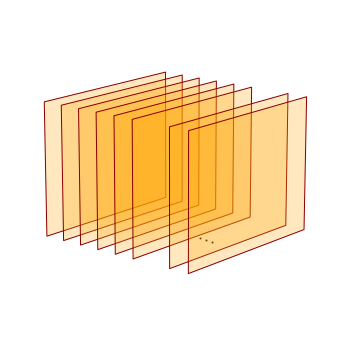
\includegraphics[width=.3\textwidth]{static/ipd.png}};

    \coordinate  (A) at (-1, -.2);
    \coordinate  (B) at (1, .5) ;
    \draw [->, thick] (A.north) to [out=90,in=180] (B.north) node [above left] {\tiny{IPD}};

    \pause

    \coordinate  (A) at (3, -1.5);
    \coordinate  (B) at (0, -2) ;
    \draw [->, thick] (A.north) to [out=-90,in=-45] (B.north) node [xshift=1.5cm, yshift=-1cm] {\tiny{strategy}};
\end{tikzpicture}
\end{document}